\documentclass[border=4pt]{standalone}
\usepackage[utf8]{inputenc}\usepackage[T1]{fontenc}\usepackage{mathptmx}
\usepackage{tikz}\usetikzlibrary{positioning,arrows.meta,calc}
\begin{document}
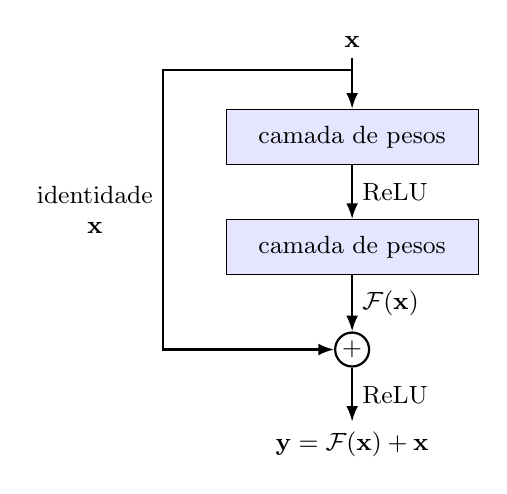
\begin{tikzpicture}[font=\small,
  box/.style={draw,fill=blue!10,minimum width=3.2cm,minimum height=0.7cm,align=center},
  arr/.style={-{Latex[length=2mm]},thick}]
\node (x) at (0,0) {$\mathbf{x}$};
\node[box] (c1) at (0,-1.2) {camada de pesos};
\node[box] (c2) at (0,-2.6) {camada de pesos};
\node[draw,circle,inner sep=1pt,thick] (sum) at (0,-3.9) {$+$};
\node (y) at (0,-5.1) {$\mathbf{y}=\mathcal{F}(\mathbf{x})+\mathbf{x}$};
\draw[arr] (x) -- (c1);
\draw[arr] (c1) -- node[right]{ReLU} (c2);
\draw[arr] (c2) -- node[right]{$\mathcal{F}(\mathbf{x})$} (sum);
\draw[arr] (sum) -- node[right]{ReLU} (y);
\draw[arr] (0,-0.35) -- (-2.4,-0.35) -- node[left,align=center]{identidade\\$\mathbf{x}$} (-2.4,-3.9) -- (sum);
\end{tikzpicture}
\end{document}
